\chapter{Literature Review}

\section{A Neural Probabilistic Language Model}
\subsection{Introduction}
Goal of statistical language modeling is to learn the joint probability function of sequences of words in a language. This is intrinsically difficult because of the curse of dimensionality. NPLM proposes to fight the curse of dimensionality by learning a distributed representation of words which allows each training sentence to inform the model about an exponential number of semantically neighboring sentences. The model learns simultaneously a distributed representation for each word along with the probability function for word sequences, expressed in terms of these representations. Generalization is obtained because a sequence of words that has never been seen before gets high probability if it is made of words that are similar to the words forming an already seen sentence. The idea of the proposed model can be summarized as follows

\begin{itemize}
    \item associate with each word in the vocabulary a distributed word feature vector (a real-valued vector in ${\rm I\!R}^m$, where m is the size of embedding vector.)
    \item express the joint probability function of word sequences in terms of the feature vectors of these words in the sequence 
    \item learn simultaneously the word feature vectors and the parameters of that probability function
\end{itemize}

\subsection{NPLM Architecture}
The basic form of the model is shown in the figure \ref{fig:Probabilistic Language Model Architecture}. The objective is to learn the function f($w_t$, $w_{t - 1}$ …., $w_{t - n}$) = P($w_t$ \(|\)  $w_1^{t - 1}$), in the sense that it gives high out-of-sample likelihood. A mapping C from any element of V to a real vector C(i) $\epsilon$ ${\rm I\!R}^m$. It represents the distributed feature vector associated with each word in the vocabulary. In practice, C is represented by a \(|\)V\(|\) x m matrix (of free parameters)

From the direct architecture figure \ref{fig:Probabilistic Language Model Architecture}, 
f(i, $w_{t - 1}$, $w_{t - 2}$…., $w_{t - n}$) = g(i, $C(w_{t - 1})$, $C(w_{t - 2})$ …, C($w_{t - n}$)). Softmax function is used in the output layer of the neural network to get the probability of the target word.

The function f is the composition of two mappings (C and g), with C being shared across all words in the context. The function g may be implemented by a feed-forward or recurrent neural network or another parameterized function, with parameters $\theta$.

\begin{figure}[H]
    \centering
    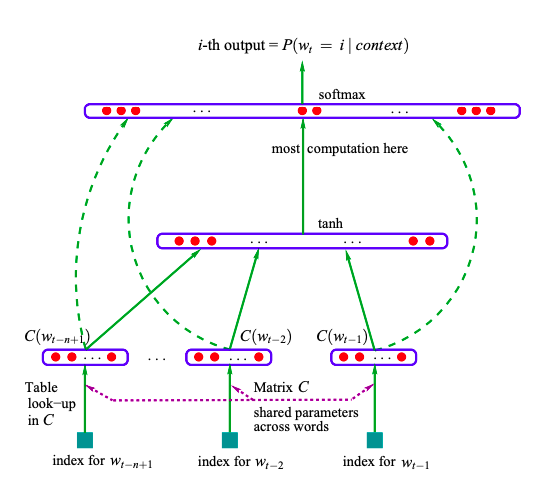
\includegraphics[scale = 0.8]{literature_review/PNLM_architecture.png}
    \caption{Direct Architecture of Probabilistic Language Model}
    \label{fig:Probabilistic Language Model Architecture}
\end{figure}

\subsection{Conclusion and Results}
The main result of this experiment is that the neural network performs much better than the smoothed trigram. Greater the length of the context words and higher the number of hidden units, the model becomes more efficient. Moreover, direct architecture was found to be better by about 2\% than the cycling architecture.

It can be deduced that the neural probabilistic model performs better due to the advantage of the learned distributed representation to fight the curse of dimensionality.

\section{Attention is all you need}
\subsection{Introduction}
Before the introduction of the transformer, the dominant sequence transduction models were based on the complex recurrent or convolutional neural networks that include an encoder and a decoder. But this paper introduced a new network architecture, the Transformer, based solely on attention mechanisms, dispensing with recurrence and convolutions entirely. Experiments on machine translation tasks show these models to be superior in quality while being more parallelizable and requiring significantly less time to train.

Attention mechanisms have become an integral part of compelling sequence modeling and transduction models in various tasks, allowing the modeling of dependencies without regard to their distance in the input or output sequences. In all but a few cases, however, such attention mechanisms are used in conjunction with a recurrent network.

\subsection{Transformer Model Architecture}
\begin{figure}[H]
    \centering
    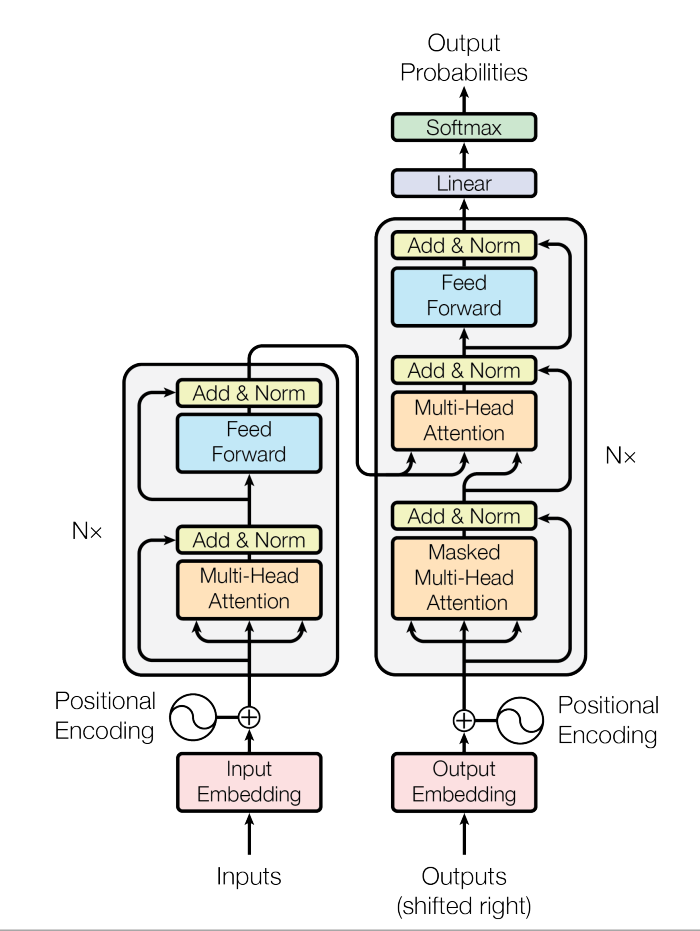
\includegraphics[scale = 0.4]{literature_review/transformer.png}
    \caption{The Transformer - model architecture}
    \label{fig:Transformer Model Architecture}
\end{figure}

\subsubsection{Encoder and Decoder Stacks}
The encoder is composed of a stack of N = 6 identical layers. Each layer has two sublayers: multi-head self-attention mechanism, and the simple position wise fully connected feed-forward network. Residual connection around each of two sub layers, followed by a layer normalization is employed in the encoder. 

The decoder is also composed of a stack of N = 6 identical layers. In addition to the two sub-layers in each encoder layer, the decoder inserts a third sub-layer, which performs multi-head attention over the output of the encoder stack. Similar to the encoder, residual connections around each of the sub layers, followed by layer normalization is employed. Self attention sub-layer in the decoder stack is modified to prevent the positions from attending to subsequent positions.

\subsubsection{Attention}
An attention function can be described as mapping a query and a set of key-value pairs to an output, where the query, keys, values and output are all vectors. The output is computed as a weighted sum of the values, where the weight assigned to each value is computed by a compatibility function of the query with the corresponding key. 

\begin{figure}[H]
    \centering
    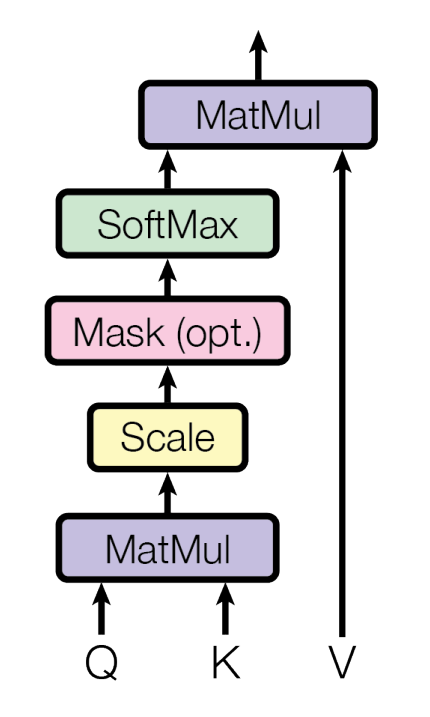
\includegraphics[scale = 0.4]{literature_review/scaled_dot_product.png}
    \caption{Scaled Dot-Product Attention}
    \label{fig:Scaled Dot-Product Attention}
\end{figure}

In scaled dot-product attention, the input consists of queries and keys of dimension $d_k$ and values of dimension $d_v$. We compute the dot products of the query with all keys, divide each by $d_k$ and apply a softmax function to obtain the weights on the values.

\begin{equation}
    Attention(Q, K, V) = softmax(\frac{QK^{T}}{\sqrt{d_k}})V
\end{equation}


In multi-head attention, instead of performing a single attention function with $d_{model}$ -dimensional keys, values and queries, we found it beneficial to linearly project the queries, keys and values h times with different, learned linear projections to $d_k$ , $d_k$ and $d_v$ dimensions, respectively. On each of these projected versions of queries, keys and values we then perform the attention function in parallel, yielding $d_v$-dimensional
output values. These are concatenated and once again projected, resulting in the final values, as depicted in figure \ref{fig:Multi-Head Attention}.

Multi-head attention allows the model to jointly attend to information from different representation subspaces at different positions. With a single attention head, averaging inhibits this.

\begin{equation}
    MultiHead(Q, K, V) = Concat(head_1, ..., head_2)W^{o}
\end{equation}

\begin{center}
    where $head_i$ = Attention($QW_i^Q$, $KW_i^K$, $VW_i^V$)
\end{center}

\begin{figure}[H]
    \centering
    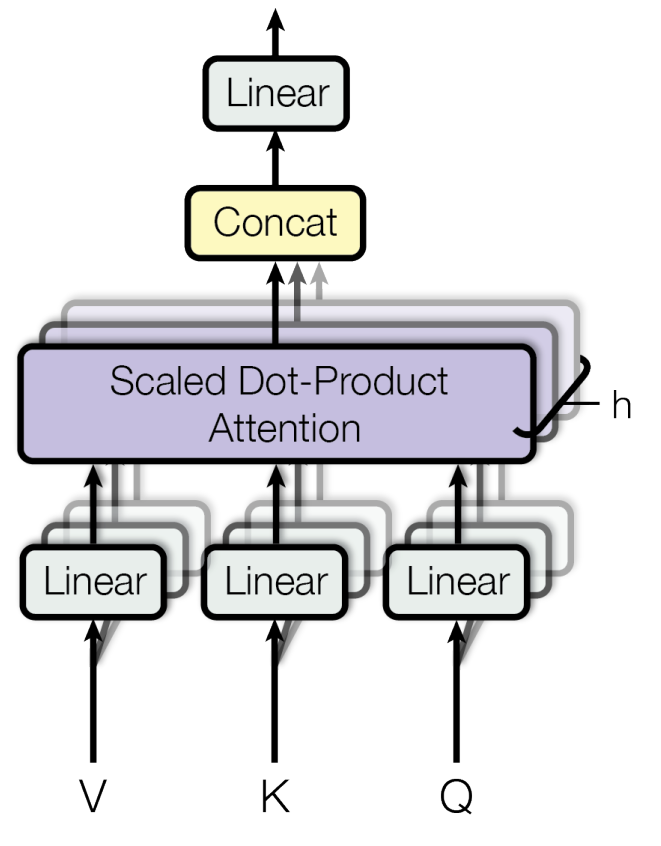
\includegraphics[scale = 0.4]{literature_review/multi_head_attention.png}
    \caption{Multi-Head Attention consists of attention layer running in parallel}
    \label{fig:Multi-Head Attention}
\end{figure}

\subsubsection{Position wise Feed Forward Neural Network}
In addition to attention sub-layers, each of the layers in our encoder and decoder contains a fully connected feed-forward network, which is applied to each position separately and identically. This consists of two linear transformations with a ReLU activation in between.

\begin{equation}
    FFN(x) = max(0, xW_1 + b_1)W_2 + b_2
\end{equation}

\subsubsection{Embedding and Softmax}
Similarly to other sequence transduction models, Learned embeddings are used to convert the input tokens and output tokens of dimension $d_{model}$. Usual learned linear transformation and softmax function are used to convert the decoder output to predict next-token probabilities. 

\subsubsection{Positional Encoding}
Since the model contains no recurrence and no convolution, in order for the model to make use of the order of the sequence, some information about the relative or absolute position of the tokens in the sequence must be injected. To this end, “positional encoding” are added to the input embeddings at the bottoms of the encoder and decoder stacks. The positional encoding have the same dimension model as the embeddings, so that the two can be summed. Sine and cosine functions of different frequencies are used for positional encoding as follows

\begin{equation}
    PE_{(pos, 2i)} = sin(\frac{pos}{10000^{2i/d_{model}}})
\end{equation}
\begin{equation}
    PE_{(pos, 2i + 1)} = cos(\frac{pos}{10000^{2i/d_{model}}})
\end{equation}

Where \textit{pos} is the position and \textit{i} is the dimension. That is, each dimension of the positinal encoding corresponds to a sinusoid.

\subsection{Conclusion and Results}
In the machine translation task, the transformer model outperformed all previous state of the art models which have used the RNNs, GRUs and LSTMs. To evaluate if the Transformer can generalize to other tasks, experiments on English constituency parsing  were performed and despite the lack of task-specific tuning, the transformer model performed surprisingly well, yielding better results than all previously reported models with the exception of the Recurrent Neural Network Grammar.

In this work, the Transformer, the first sequence transduction model based entirely on attention, replacing the recurrent layers most commonly used in encoder-decoder architectures with multi-headed self-attention is presented.

Till today, various transformer models have been developed which have performed better on all kinds of natural language processing tasks like language modeling, text classifications, questions answering, machine translation, sentence similarity, summarization, etc.

\section{Nepali Spelling Correction}
In the pre-computer era, spelling correction was primarily a manual process. Dictionaries and grammar books were used to verify correct spellings, and proofreaders manually identified and corrected spelling errors in written texts. With the advent of computers, rule-based spelling correction systems emerged. These systems relied on predefined rules to identify and correct spelling mistakes. Rules were typically based on common spelling patterns, phonetics, and grammatical rules. One phonetical rule-based algorithm is Soundex Algorithm. However, these early systems had limited effectiveness due to the vast number of language-specific exceptions and irregularities. Another set of algorithms is based on a combination of dictionary-based and rule-based. For example, Hanspell is a dictionary-based spelling correction engine that applies certain transformations to find the rank of candidate words in a dictionary to make predictions for the correct spelling.

Apart from using rules, statistical methods are also popular. These approaches used large corpora of correctly spelled words to estimate the likelihood of different word sequences. By comparing input words to these statistical models, spelling errors could be identified, and suggestions for corrections generated. Early statistical models often used n-gram language models and algorithms like the noisy channel model.
The noisy channel model, though developed by Shannon in 1948, was first proposed for spelling correction in IBM Watson Research(Mays et al., 1991) and at Bell Laboratories (Kernighan et al. 1990) with the idea of combining prior and likelihood.

One can use statistical models to utilize corpora of unlabeled text to build both the likelihood model(error model) and the prior. Whitelaw et al.(2009), used huge texts of web pages to train the n-gram, prior model. They used a partitioning-based likelihood model developed by Brill and Moore(2000). In this approach, words were partitioned into substrings and the substrings were aligned with the possible correct word. The simple counting-based probability can be calculated for all such substrings using triples of the correct word, misspelled word, and frequency extracted from the corpus in an unsupervised way. The approximate likelihood probability can then be calculated by multiplying all probability values for the substring.

\section{Nepali Speech Recognition Using CNN, GRU, and CTC}
This paper presents an idea to build the Nepali ASR system to convert the spoken Nepali language to its textual representation using a CNN, GRU, and CTC model. The features in the raw audio are extracted by using the MFCC algorithm. MFCC features are a sequence of Acoustic feature vectors where each vector represents information in a small-time window of the signal. CNN is used to capture high-level spatial features from the image. The plot of MFCC can be viewed as a transformed intensity of frequencies over time which resembles images, hence CNN can be used to capture high-level features in the spatial domain. GRU is responsible for constructing the acoustic model. The decoding is carried out using a CTC network. The CTC is based on Bayes’ decision theory. It receives output from the softmax function. 


\begin{figure}[H]
    \centering
    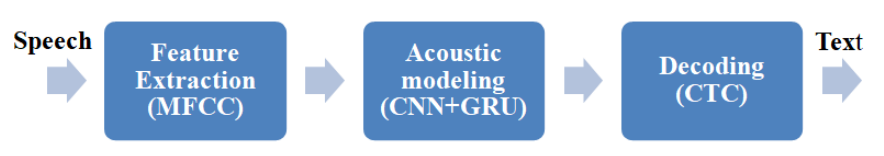
\includegraphics[scale = 0.4]{literature_review/architecture_proposed_asr.png}
    \caption{Architecture of proposed ASR system}
    \label{fig:Architecture of proposed ASR system}
\end{figure}

The experimental setup is carried out on the GPU MX150. For the pre-processing, feature extraction, training, and testing, python and its library have been used. The obtained results from various experiments were as follows

\begin{figure}[H]
    \centering
    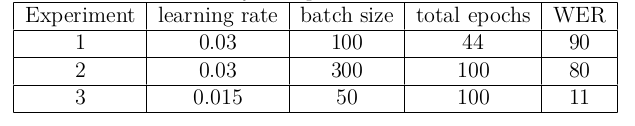
\includegraphics[scale = 0.4]{literature_review/asr_experiment_summary.png}
    \caption{Summary of experiments with the results}
    \label{fig:Summary of experiments with the results}
\end{figure}

